% Drawing 156-8/06-4 -- folder 156-8, batch 06, archive page 119 (PDF page 120).
% Transcription: la même figure qu'en p.~118 : un point plein $a$, un point ouvert en $b$, un point plein entre parenthèses en $c$, un crochet en $d$, un point isolé $e$.
% Kind: configuration on a line (point types). Method 3 (encoded, rendered from the data). Status: ok.
% Notes: The same figure as p. 118 (06-3), redrawn: same encoding, checked identical.
% Coordinates: 1 unit = 1 mm = 1/100 of the crop width (bbox in page fractions: [0.15, 0.26, 0.62, 0.3]).
% Redrawn by Claude (claude-opus-5-5), issue #73 pilot, 2026-11-07; not checked by a human; not compiled (no TeX in the session).
% Rights: reproduces part of the work -- behind RENDER_TRANSCRIPTS, never published by itself.
\documentclass[tikz,border=3pt]{standalone}
\usepackage{amsmath,amssymb}
\usetikzlibrary{patterns,arrows.meta}
\tikzset{pencil/.style={black!45}, struck/.style={black!35}, mark/.style={circle,draw,inner sep=1.3pt}, pt/.style={circle,fill,inner sep=0.9pt}, opt/.style={circle,draw,fill=white,inner sep=1.1pt}}
\begin{document}
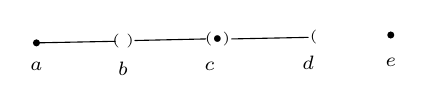
\begin{tikzpicture}[x=1mm,y=1mm,line cap=round,line join=round,font=\scriptsize]
\node[pt] at (31,-6.5) {};
\draw (31,-6.5) -- (41,-6.3);
\node[inner sep=1pt] at (42,-6.3) {\tiny $(\ )$};
\draw (43.5,-6.2) -- (52.5,-6);
\node[inner sep=1pt] at (54,-6) {\tiny $(\bullet)$};
\draw (55.8,-6) -- (65.5,-5.8);
\node[inner sep=1pt] at (66.2,-5.8) {\tiny $($};
\node[pt] at (76,-5.5) {};
\node[inner sep=1pt] at (31,-9.5) {\scriptsize $a$};
\node[inner sep=1pt] at (42,-9.8) {\scriptsize $b$};
\node[inner sep=1pt] at (53,-9.5) {\scriptsize $c$};
\node[inner sep=1pt] at (65.5,-9) {\scriptsize $d$};
\node[inner sep=1pt] at (76,-9) {\scriptsize $e$};
\end{tikzpicture}
\end{document}
